\section{Client-server view (UML Component diagram)}\label{sec:client-server}
In Figure \ref{fig:cc-context}, we present a context diagram of the client-server view, detailing the external communication to and from the system. The entry points to the system are the (mostly automated) external version of raw data submission. The Customer Organisation and/or Social Secretary can submit Raw Data Batches via the specified protocols supported by the eDocs system.
The other entry point being the \ttt{UIfacade}, which is contacted by User Software for User Interface Actions, e.g. a management dashboard for the Customer Administrator (one or more per Organisation) to query for job statuses, or a log-in system for recipients to log in to the PDS.
The exit points of the system are more versatile. There is one closely related to the UI Actions, where parts of the system respond to queries by directly supplying information to the user sessions, which in turn are individual (dedicated) intermediaries for instances of the client software. This bypasses the \ttt{UIFacade} as a bottleneck.
The \ttt{SubmissionSubsystem} queries an \ttt{External Information Broker} when verifying the meta-data of Raw Data Batches and Entries as specified in \emph{UC3}.
The \ttt{BillingSubsystem} contacts the \ttt{Billing System} (external of the actual eDocs system) used by the eDocs Company periodically to bill users of eDocs.
The \ttt{CommunicationSubsystem} submits composed e-mails to an \ttt{External Email Provider} for delivery. This functionality is used for reporting errors in the system to the eDocs admin, various notifications to CO admins, delivery of documents etc.
There are two other external communication mechanisms for document delivery, namely the \ttt{Zoomit} service's \ttt{Document Delivery} interface and the \ttt{Print \& Postal Service}'s one. These are both directly used by the delivery subsystem, in contrast to document delivery by e-mail, which passes through the \ttt{CommunicationSubsystem}, as explained earlier.

\begin{figure}[!htp]
    \centering
    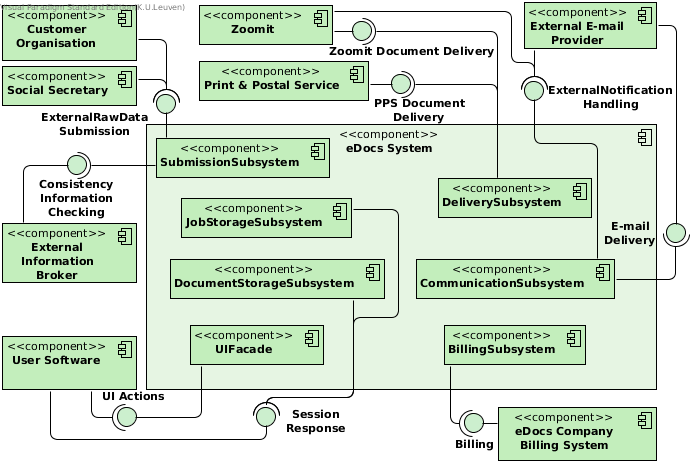
\includegraphics[width=\textwidth]{figures/Context Diagram 1.png}
    %\missingfigure[figwidth=0.8\textwidth]{Context diagram of the client-server view.}
    \caption{Context diagram for the client-server view.}\label{fig:cc-context}
\end{figure}

Figure \ref{fig:cs-primary} shows the primary component-and-connector diagram of the system. The presented overview divides the eDocs system into several subsystems, each with their dedicated functionalitie(s). The division are straightforward, and make for a less coupled system.\\
The \ttt{SubmissionSubsystem} accepts \ttt{Raw data batches} from an external user or via the \ttt{UIFacade}. It verifies these \ttt{Batches} and then registers them for generation in the \ttt{JobStorageSubsystem} and the \ttt{DocumentGenerationSubsystem}.\\
The \ttt{JobStorageSubsystem} stores the statuses of document generation and delivery jobs. It records raw data for document generation until said document has been succesfully generated succesfully. The \ttt{Subsystem} can be queried for job statuses, e.g. by the administrator of a Customer Organisation. It is contacted by the different subsystems concerned with the lifecycle of a document in the system, to record and update the document's status e.g. Waiting for generation, generated, delivered etc.\\
The \ttt{DocumentGenerationSubsystem} \\
The \ttt{GeneratedDocumentHandler} is a passthrough point for generated documents. This component is not an actual subsystem, but an important branching point in the internal document flow. The \ttt{GeneratedDocumentHandler} determines for a document exactly where it has to go (e.g. whether e-mail actually means e-mail or should go to the PDS), and submits the document with the specific addressing data to both the \ttt{DeliverySubsystem} and the \ttt{DocumentStorageSubsystem}. It also marks a document as generated in the \ttt{JobStorageSubsystem}.\\
The \ttt{DocumentStorageSubsystem} \\
The \ttt{DeliverySubsystem} performs the actual document delivery (or notification of a new document) to recipients. It manages all \ttt{Delivery Channels} and determines from the addressing data by the \ttt{GeneratedDocumentHandler} which \ttt{Channel} to use for delivery. It directly addresses the used external service for delivery (e.g. Zoomit, Print \& Postal Service), except in the case of email delivery. Composed delivery or notification e-mails are passed to and delivered by the \ttt{CommunicationSubsystem}.\\
The \ttt{CommunicationSubsystem} \\
The \ttt{UserManagementSubsystem} stores all information regarding the different types of users and registered (non-authenticable) entities , which currently are: Recipients, Customer Administrators, actual Customer Organisations and eDocs Administrators. For the authenticable users, the \ttt{UserManagementSubsystem} provides authentication and authorization functionality, in turn supported by session logic in the \ttt{UIFacade}. The \ttt{Subsystem} provides functionality for the system to query info about Recipients, Customer organisations etc. and add or update this information (mostly by the eDocs administrator). Since the \ttt{UserManagementSubsystem} also governs whether a recipient is \emph{Registered} or not, the \ttt{Subsystem} notifies the \ttt{DocumentStorageSubsystem} to add or remove a recipient's documents in the PDS system.\\
The \ttt{BillingSubsystem} \\
The \ttt{LookupSubsystem} \\
The \ttt{UIFacade} acts as an intermediary between all different kinds of user interfaces (a management dashboard, a Recipient PDS client etc.) and the system. The \ttt{UIFacade} passes all calls to the actual subsystems. It has a session infrastructure for user interface clients, so it is not one single bottleneck for all requests. The current different functionalities handled by the \ttt{UIFacade} are loging users in and out, registering new users, looking up job statuses and documents, submitting raw data through a dashboard and entering system information for load balancing in lookups.\\

\begin{figure}[!htp]
    \centering
    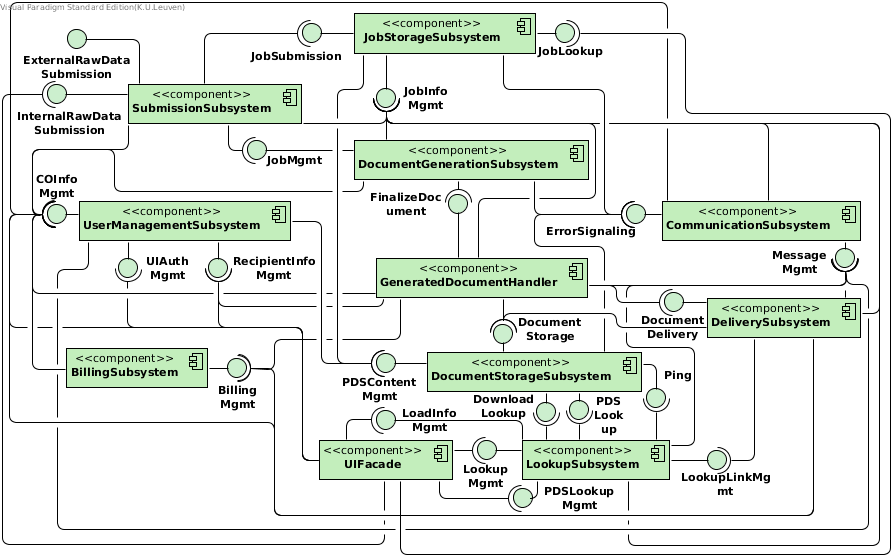
\includegraphics[width=\textwidth]{figures/Subsystem Diagram.png}
    %\missingfigure[figwidth=0.8\textwidth]{Primary diagram of the client-server view.}
    \caption{Primary component-and-connector view of the proposed architecture.}\label{fig:cs-primary}
\end{figure}

\subsection{Main architectural decisions}
Discuss your architectural decisions for the most important requirements in
more detail using the components of the client-server view.
Pay attention to the solutions that you employed and the alternatives that you
considered.
The explanation here must be self-contained and complete.
Imagine you had to describe how the architecture supports the core
functionality to someone that is looking at the client-server view only.
Hide unnecessary details (these should be shown in the decomposition view).

\subsubsection{ReqX\@: requirement name}
Describe the design choices related to \emph{ReqX} together with the rationale
of why these choices where made.

\subsubsection*{Alternatives considered}
\paragraph{Alternative(s) for choice 1} Explain what alternative(s) you
considered for this design choice and why they where not selected.
